\documentclass[10pt]{article}
% \def\StudentVersion{}
\usepackage{../../common}
\makeatletter

\def\LecStr{Alexander Rush}
\def\LecNum{1}
\def\LecTitle{Lectures Notes on CSP}
\def\LecDate{}


\begin{document}
\MakeScribeTop{}

\section{Board 0}

\begin{figure}[h]
  \centering
  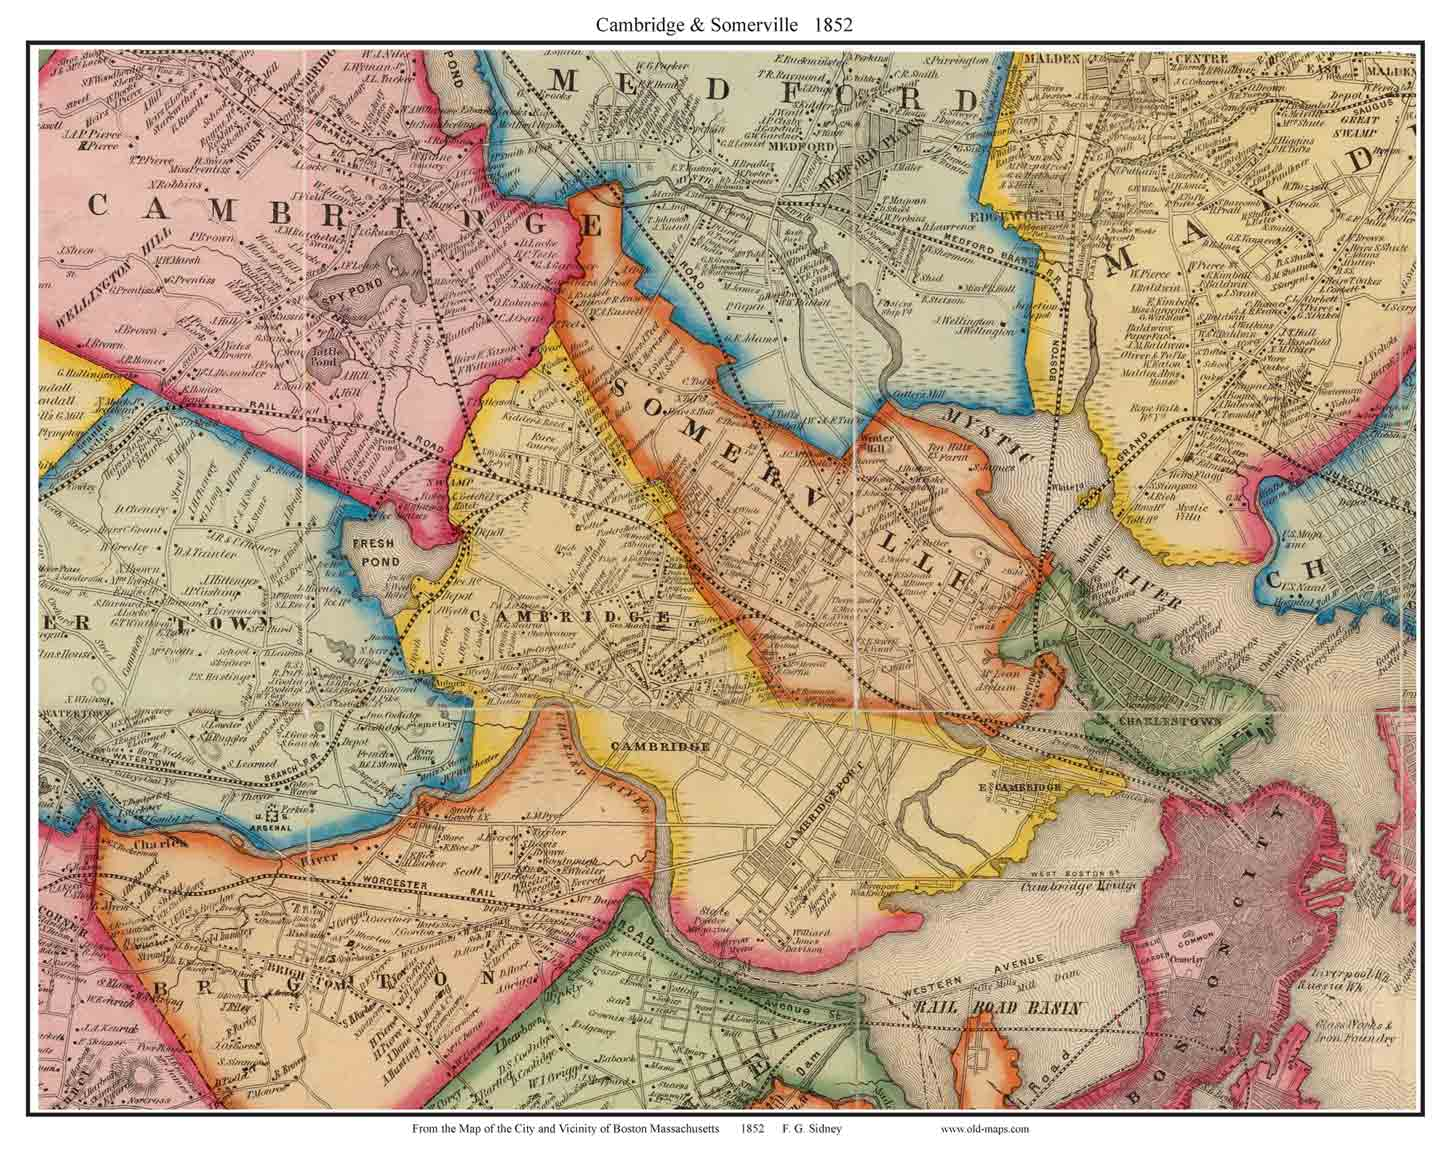
\includegraphics[width=0.8\linewidth]{../pics/CambridgeSomerville_1852_web}
  \label{fig:camb}
  \caption{Cambridge-area circa 1852. Best viewed in color.}
\end{figure}

\section{Summary}

\begin{itemize}
\item CSP Formalism
\item Assignments 
\item Factor graphs
\item Examples:
  \begin{itemize}
  \item Graph Checking
  \item Part-of-Speech Tagging
  \end{itemize}
\item Consistency Checking
\end{itemize}

\section{Board 1}

Constraint Satisfaction Problem (CSP)

\begin{itemize}
\item Explicit representation of problem (not just ``actions'')
\item Can use search, but generate heuristics/ordering automatically
\item Very general/useful class of search problems  
\end{itemize}

\section{Board 2}

% We will apply this approach to a map of the Cambridge area
% shown below. For this problem we will define the coloring set as

Graph Coloring.

\begin{itemize}
\item Scheduling problems (jobs, class, hiring, Starcraft build-order) 
\item Compiler theory (register allocation)
\item Map-making? (apparently not)
\end{itemize}

 $\msc{Colors} = \{\mathrm{R, Y, O, B}\}$, i.e. red, yellow, orange, and blue. Specify
a valid coloring relationship using set notation: 

\[\msc{DifColor} = \{c_1, c_2 \in \msc{Color} : c_1 \neq c_2 \}\].

-Declarative specification of problem. 

\section{Board 3}


A constraint satisfaction problem (CSP) defines a sets of \textbf{variables} which are jointly constrained. Formally a constraint satisfaction problem is defined by the following elements:

Factor Graph formulation

 \air
\begin{center}
\begin{tabularx}{\linewidth}{llX}
  \toprule
  Name (AIMA) & Type & Description \\
  \midrule
\\
 Variables & $X_1, \ldots, X_n$ &  The variables of the CSP .\\\\
 Variable Domains & $\mcD_1, \ldots, \mcD_n$&   The set of labels for each var can 
 \midrule\\
 Factors & $F_1, \ldots,F_m$ &  The factors of the CSP. Each factor constrains variable(s)
 Factor Domains &  $\mcR_1, \ldots, \mcR_m$ & The set of labels the variable constrained by a factor can take on. 
 \bottomrule
\end{tabularx}
\end{center}

\section{Board 4}
As an example, say we have three variables 
- Variables: $X_1, X_2, X_3$
- Domains: $\mcD_1 = \mcD_2 = \mcD_3 = \{\mathrm{A, B, C}\}$. 

- Factor $F_1 = (X_1, X_3)$

- Factor Constraint - $\mcR_1 = \{(\mathrm{A, B}), \mathrm{(A, C})\} \rangle $

The
only two valid labels for $X_1$ and $X_3$ are $X_1 = A, X_3 = B$ and
$X_1 = A, X_3=C$. 

- It says nothing about $X_2$.  

``Arc'' : a factor that only constraint two variables.
% While a single factor
% can constrain many variables, we will mainly consider
% pairwise factors, also known as \textbf{arcs}.

% , constrained by that factor, for example $F_2 = ( X_1, X_4, X_{10})$  \\\\
% $\mcR_i$ corresponds to factor $F_i$ for all $i \in \{1, \ldots, m\} $.     \\\\

\section{Board 5: Big}

Instead of paths as in search, we will be interested in assignments for CSP. In particular:  

\begin{defn}
An \textbf{assignment}, $X_1 = (\mcD_1 \cup \{\epsilon\}) \times \ldots \times (\mcD_n \cup \{\epsilon\})$ consists of a label (or blank) for each variable. We say the assignment is \textbf{partial} if it includes $\epsilon$, and \textbf{complete} if it does not. 
\end{defn}


\begin{defn}
  A partial/complete assignment is \textbf{consistent} if it
  does not violate any constraints. That is for each factor $(X_i, X_j)$,
  the assignment is $(A_i, A_j)$ is in the set of valid relations or
  at least one is $\epsilon$.
\end{defn}

A complete, consistent assignments is analogous to a solution path.
For CSPs, we will treat all consistent paths as equally acceptable,
i.e. there is no costs associated with assignments. (Note, however
there are important variants of the CSP formalism that do model this
idea of an assignment costs.)

\section{Board 6}

Instead of paths as in search, we will be interested in assignments for CSP. In particular:  

\begin{defn}
A \textbf{assignment} $A_1 \in (\mcD_1 \cup \{\epsilon\}) \times \ldots \times A_n (\mcD_n \cup \{\epsilon\})$ consists of a label (or blank) for each variable. We say the assignment is \textbf{partial} if it includes $\epsilon$, and \textbf{complete} if it does not. 
\end{defn}


\begin{defn}
  A partial/complete assignment is \textbf{consistent} if it
  does not violate any constraints. That is for each factor $F$ that constraint $X_i, X_j$,
  the assignment is $A_i$ $A_j$ is in the set of valid relations or
  at least one is $\epsilon$.
\end{defn}

A complete, consistent assignment is analogous to a solution path.
For CSPs, we will treat all consistent paths as equally acceptable,
i.e. there is no costs associated with assignments.

 (Note, however
there are important variants of the CSP formalism that do model this
idea of an assignment costs.)

\section{Board 7}


 \air
\begin{center}
\begin{tabularx}{\linewidth}{lX}
  \toprule
 Variables & \censor{$X = \langle \mathrm{Cambridge, Somerville, Brighton, Boston, Watertown} \rangle$}   \\\\
 Labels & \censor{$\mcD_1 = \msc{Colors}, \ldots, \mcD_n = \msc{Colors}$}   \\\\
 \midrule \\ 
 Factors & \censor{\begin{eqnarray*}
   F_1 &= & (\mathrm{Cambridge, Somerville}),\\
   F_2 &= &(\mathrm{Cambridge, Boston}), \\  
   F_3 &= &(\mathrm{Cambridge, Watertown}),  \\  
   F_4 &= &(\mathrm{Cambridge, Brighton}), \\ 
   F_5 &= &(\mathrm{Brighton, Boston}), \\  
   F_6 &= & (\mathrm{Brighton, Watertown})  
   \end{eqnarray*}} \\\\
 Constraints &  \censor{$\mcR_1 = \msc{DifColor},  \ldots, \mcR_6 = \msc{DifColor} $}  \\\\
 \bottomrule
\end{tabularx}
\end{center}
\air

So for this problem are $n= 5$ variables and $m=6$ factors, each is also an arc. The representation is much easier to visualize as a factor graph. Below we shows a factor graph representation of the same CSP. 
However note it does not explicitly show the constraints of the graph. 

\section{Board 8}

Factor Graph (Constraint Hypergraph)

- Undirected graph 
- bipartite: two types of nodes, only edges between.

- variable nodes ($n$, drawn as circles)
- factor nodes ($m$, drawn as squares)

- Connections for $F_i= (X_{f_1}, \ldots, X_{f_o})$ between

- No representation of variable or factor domains  

\section{Board 9}
\air
\begin{figure}[h]
  \centering
  \begin{tikzpicture}
    \draw node(s)[draw, ellipse] at (2.5, 2.5){Somerville};
    \draw node(w)[draw, ellipse] at (-5, 0){Watertown};
    \draw node(c)[draw, ellipse] at (0, 0){Cambridge};
    \draw node(br)[draw, ellipse] at (-2, -2.5){Brighton};
    \draw node(bo)[draw, ellipse] at (2.5, -2.5){Boston};
    \draw (br) -- node[draw, fill]{} (c);
    \draw (br) -- node[draw, fill]{} (w);
    \draw (c) -- node[draw, fill]{} (s);
    \draw (c) -- node[draw, fill]{} (w);
    \draw (br) -- node[draw, fill]{} (c);
    \draw (c) -- node[draw, fill]{} (bo);
    \draw (br) -- node[draw, fill]{} (bo);
    
  \end{tikzpicture}
  \label{fig:cambfactor}
  \caption{Factor graph showing the constraints for the Cambridge 
  graph coloring problem. }
\end{figure}
\air



\section{Board 10}

\begin{exercise}
  Generate: 

  \begin{enumerate}
  \item A complete, consistent assignment for this problem.
  \item An incomplete, consistent assignment for this problem.
  \item An complete, inconsistent assignment for this problem.
  \end{enumerate}
\end{exercise}

\censor{
\begin{enumerate}
\item A complete, consistent assignment is show in Figure~\ref{fig:camb}. In our notation this assignment is represented as $\langle \mathrm{Y, O, O, G, B} \rangle$.
\item   If we had the same graph, but had not yet assigned a color to Cambridge we would write it as $\langle \epsilon, \mathrm{ O, O, G, B} \rangle$. This assignment is incomplete, but consistent.
\item  Alternatively if we flip the color of Cambridge and Somerville we end up with  $\langle \epsilon, \mathrm{O, Y, O, G, B} \rangle$ which is complete but inconsistent.
\end{enumerate}
}

\section{Board 11}
Example 2.

SIRI. 

Let's consider a rather different example from the field of natural 
language processing. Imagine we are implementing a system like SIRI
and we are given a crucial question such as ``Where is Toscanini's located?''.
One of the first steps for handling such a question is to label each word 
with its part-of-speech tag. 


\section{Board 12}
\begin{enumerate}
\item Tag Dictionary: Each tag is a match its word $\msc{TagDict}$ 
\item Neighbor Tags: Neighboring tags are consistent $\msc{TagCons}$
\end{enumerate}

The first constraint will ensure that the tag of each word is consistent
with the tags previously seen for that word. Many words in English are consistent 
with several different tags.  The second constraint will ensure that the 
tag sequence is consistent with what is common in English.

If we can find a complete consistent assignment here, it is likely to
give a good tagging of the sentence.

  \scalebox{0.8}{
  \begin{tikzpicture}
    \draw node(ta)[draw, ellipse] at (0, 1){Tag1};
    \draw node(tb)[draw, ellipse] at (5, 1){Tag2};
    \draw node(tc)[draw, ellipse] at (10, 1){Tag3};
    \draw node(td)[draw, ellipse] at (15, 1){Tag4};

    \draw node(wa)[draw, ellipse] at (0, -1){Word1 (\textit{Where}) };
    \draw node(wb)[draw, ellipse] at (5, -1){Word2 (\textit{is})};
    \draw node(wc)[draw, ellipse] at (10, -1){Word3 (\textit{Toscanini's})};
    \draw node(wd)[draw, ellipse] at (15, -1){Word4 (\textit{located?})};
    
    \draw (ta) -- node[draw, fill]{} (tb);
    \draw (tb) -- node[draw, fill]{} (tc);
    \draw (tc) -- node[draw, fill]{} (td);
    \draw (ta) -- node[draw, fill]{} (tb);

    \draw (ta) -- node[draw, color=blue,fill]{} (wa);
    \draw (tb) -- node[draw, color=blue,fill]{} (wb);
    \draw (tc) -- node[draw, color=blue,fill]{} (wc);
    \draw (td) -- node[draw, color=blue,fill]{} (wd);

  \end{tikzpicture}
}

  \begin{itemize}
  \item The word 'is' most always be a verb.
  \item The Adj/Noun
  \end{itemize}

In practice there is a score.

\section{Board 13}
Inference

What do we know about our variables based on the current information?

- limit domains of variables based on knowledge.

- ``consistency'' check. If there a possible consistent assignment?     

\section{Board 14}

Cambridge, Somerville, Brighton, Boston, Watertown
\[\langle \epsilon, \epsilon, \mathrm{O, G, B} \rangle\]

Draw colors


\section{Board 15}
The algorithm proceeds as follows: 

\begin{enumerate}
\item Somerville-Cambridge factor 
\item  check whether any of it constrains out any of Somerville's assignments. 
  However since the Cambridge variable could at this point be any 
  color, we cannot limit out any of the coloring options for Somerville.
\item Check around Cambridge. 
  \begin{itemize}
  \item    the factor with Watertown means it cannot be blue, 
  \item the factor with Brighton means it cannot be orange, 
  \item the factor with Boston means it cannot be green. 
  \end{itemize}
  This limits the domain $\mcD_1$ from $\{\mathrm{R,Y, O, B }\}$ to $\{\mathrm{Y}\}$

\item Changed Cambridge, recheck
  . This means we return
  to the Somerville-Cambridge constraint. However now we know the
  domain of Cambridge is $\{\mathrm{Y}\}$ which limits the domain of
  Somerville $\mcD_2$ to $\{\mathrm{R, O, B }\}$
\end{enumerate}

\noindent For this particular problem after the consistency checks it is now easy to find a complete consistent assignment. 

\section{Board 16}

\subsection{Arc Consistency}

When all factors are of size 2, this technique of enforcing consistent
domains is known as \textbf{arc consistency}. The algorithm is shown
below. Note for the purpose of this algorithm we treat the partial
assignment as a domain of size one (i.e. Watertown would have domain
$\{\mathrm{B}\}$ ).

\begin{algorithm}[h]

\begin{algorithmic}[1]

  \Procedure{ArcConsistency}{}
  \State{queue $\gets [F_1, F_2, \ldots F_m]$}
  \While{queue is not empty}
  \State{$F_i \gets$ queue.pop() }
  \State{$(X_j, X_k) \gets F_i$ }
  \State{rev $\gets$ false}
  \For{$x \in \mcD_j$}
  \If{\censor{for all $y \in \mcD_k$, $(x, y) \not \in \mcR_i$}}
  \State{$\mcD_j \gets$ \censorm{$\mcD_j \setminus\{x\}$}}
  \State{rev $\gets$ true}
  \EndIf{}
  \EndFor{}
  \If{rev}
  \If{$\mcD_i$ is empty}
  \Return{false}
  \EndIf{}
  \For{\censorm{factors $F$ neighboring $X_j$}}
  \State{queue.push($F$)}
  \EndFor{}
  \EndIf{}
  \EndWhile{}
  \State{\Return{true}}
  \EndProcedure{}
\end{algorithmic}
\end{algorithm}

\section{Board 17}

By itself, this algorithm is not guaranteed to find a complete consistent assignment. In fact, if we run the algorithm on a blank assignment for graph coloring it, will not even limit the domain at all! However it can be very effective for other problems, for instance for the tagging example. 

\begin{exercise}
  What is the complexity of running this algorithm?
\end{exercise}

\section{Board 18}

\subsection{Forward Checking}

For arc consistency we include a check that the domain $\mcD_i$ is
empty. When run from the initial assignment we would hope that this
check is never hit (or else the problem is unsolvable). However, we
can also use arc consistency to \textbf{forward check} whether consistent, 
incomplete assignments are on the right path. 

To do this, we set $\mcD_i = \{A_i\}$ for all $i$ such that
$A_i \neq \epsilon$.  We then run the arc consistency algorithm. If
the algorithm returns false, it tells use that there is no consistent,
complete assignment that overlaps with $A$. As we assign, new
variables we can repeat this check, starting with the factors that
constrain the newly assigned variable. We will see in the homework
that this is an important tool for speeding up CSP search.

\section{Board 19}

\end{document}